\chapter{Поток частиц в трубе}

	\section{Теоретическое введение}
	
		В цилиндрической трубе с поперечным сечением $ S $ движутся частицы вещества (пылинки, электроны). 
		Скорость их движения $ u(t) > 0 $
		вдоль оси $ x $, вообще говоря, изменяется со временем.
		Например, заряженные частицы могут 
		ускоряться или замедляться под
		действием электрического поля. Для
		построения простейшей модели 
		рассматриваемого движения введем следующие предположения\cite{Samarskiy}:
		
		\begin{enumerate}
			\item \label{it:1}  Частицы между собой не взаимодействуют (не сталкиваются, не притягиваются и т. д.). Для этого, очевидно, плотность частиц должна быть достаточно малой (в этом случае заряженные частицы не только не сталкиваются, но и не оказывают друг на друга влияния из-за большого расстояния между ними).
		
			\item \label{it:2} начальная скорость всех частиц, находящихся в одном и том же поперечном сечении с координатой $ x $, одинакова и направлена вдоль оси $ x $;
		
			\item \label{it:3} начальная плотность частиц также зависит только от координаты $ x $;
		
			\item \label{it:4} внешние силы, действующие на частицы, направлены вдоль оси $ x $.
		\end{enumerate}
		
		Предположение \ref{it:1} означает, что скорость частиц может изменяться лишь под действием внешних сил, предположения \ref{it:2}-\ref{it:4} обеспечивают одномерность процесса переноса, т. е. зависимость искомой плотности потока частиц только от координаты $ x $ и времени $ t\le 0 $.
		
		Итак, по заданной начальной плотности $ р(x,t=0)= p_0(x) $  необходимо
		найти плотность частиц $ p(x,t) $ в любой момент времени для 
		любых $ x $ (скорость движения u(t) задана). 
		Прибегнем к закону сохранения массы, подсчитав баланс вещества в
		малом элементе трубы от $ x $ до $ x+dx $ за время $ dt $. 
		Слева в элементарный объем входит количество вещества с массой,
		равной
		
		
		\begin{equation}
		S u(t) dt p(x,t+ \xi dt), 0 \le  \xi  \le 1, 
		\end{equation}
		
		где $ S u(t) dt $ — объем вошедшего за 
		промежуток времени $ dt $ вещества. Через правое
		сечение элемента за то же время выходит масса, равная
		\begin{equation}
		 -Su(t)dtp(x+dx,t+\xi'dt), 0\le\xi'\le1,
		\end{equation}
		т. е. суммарное изменение массы равно
		\begin{equation}
		 dm = S u(t) (p(x,t+ \xi  dt)-p(x+dx,t+ \xi ' dt)) dt.
		\end{equation}
		В силу малости промежутка $ dt $ скорость $ u(t) $ считается постоянной. 
		Величины $ p(x,t+ \xi  dt) $ и $ p(x+dx,t+ \xi ' dt) $ — средние по времени значения
		плотности в сечениях $ x $ и $ x+dx $.
		
		Другой способ подсчета изменений в фиксированном объеме $ S dx $ ст
		очевиден из смысла величины $ p(x,t) $:
		
		\begin{equation} dm = S (p(x+ \eta dx,t+dt)-p(x+ \eta 'dx,t)) dt, 0< \eta , \eta '<1 \end{equation} 
		
		где $ (p(x+ \eta dx,t+dt) $ и $ p(x+ \eta 'dx,t) $ — средние по пространству 
		значения плотности в моменты $ t $ и $ t+dt $.
		
		Приравнивая оба полученные для $ dm $ выражения и устремляя $ dx $
		и $ dt $ к нулю, приходим к уравнению для $ p(x,t) $, отвечающему закону
		сохранения массы,
		
		\begin{equation} \frac{dp}{dt}+\frac{dp}{dx}u(t)=0, -\infty<x<\infty, t>0, \label{eq:1}\end{equation} 
		
		c начальным условием
		
		\begin{equation} p(x,0)=p_0(x), -\infty <x< \infty \label{eq:2}\end{equation} 
		
		Величина $ pu $ (поток вещества, или поток массы) равна 
		количеству вещества, проходящему в единицу времени через единичную
		поверхность поперечного сечения трубы. Как видно из \ref{eq:1}, скорость
		изменения плотности вещества со временем в любом сечении 
		определяется «скоростью» изменения потока вещества по координате $ x $.
		Схожим свойством обладают многие модели, отвечающие законам 
		сохранения и описывающие совсем другие процессы.
		
		В случае постоянной скорости $ u(t) = u_0 $ приходим к простейшему
		линейному уравнению в частных производных
		
		
		\begin{equation} 
			\frac{dp}{dt} + u_0 \frac{dp}{dx} = 0, -\infty<x<\infty, t>0, 
			\label{eq:3} 
		\end{equation} 
		
		Его общее решение нетрудно найти, приняв во внимание, что
		уравнение \ref{eq:3} имеет характеристики — линии $ x = u_0 t + C $, на
		которых значения искомой функции постоянны во времени, т. е.
		$p(x=u_0 t + C,t) = p_c$, или, в эквивалентной записи,
		
		\begin{equation} p(x,t) = p(x+u_0 (t - t_0), t_0),  t - t_0 \ge 0 \end{equation}
		
		Выбирая $ t_0 = 0 $, получим
		
		\begin{equation} p(x,t) = p( \xi ) = p(x + u_0 t).  \label{eq:4} \end{equation}
		
		Интеграл \ref{eq:4} и является общим решением уравнения \ref{eq:3}. 
		Из формулы \ref{eq:4} и начальных данных \ref{eq:2} легко найти искомую функцию, 
		причем она зависит не по отдельности от переменных $ x, t $, 
		а от их комбинации $  \xi  = x + u_0 t$ (бегущая волна).
		Пространственный профиль плотности без 
		искажений переносится вдоль потока 
		с постоянной скоростью 
		(уравнение \ref{eq:3} называют также уравнением переноса). 
		Это основное свойство решения уравнения \ref{eq:3} 
		несколько модифицируется в случае,
		когда скорость частиц зависит от времени — профиль плотности 
		переносится за равные промежутки времени на разные расстояния.
		В этом случае $  \xi  = \int^t_0  u(t) dt$.

	\section{Реализация}
	
		Реализация производилась на языке Java, версия 1.8. В программе присутствует секция с общей информацией о модели \ref{fig:tubetheory} и секция с интерактивным примером \ref{fig:tubeexample}, в которой дано графическое представление модели, а при изменении параметров появляются обучающие подсказки. Исходный код модели доступен на \href{https://github.com/goto1134/mathmodels}{GitHub}.
	
		\begin{figure}[th]
			\centering
			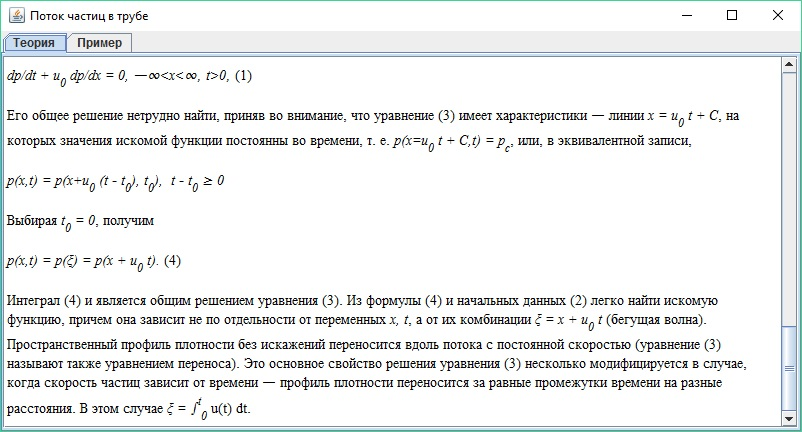
\includegraphics[width=0.7\linewidth]{images/tube_theory}
			\caption{Общая информация о модели}
			\label{fig:tubetheory}
		\end{figure}
	
		\begin{figure}[th]
			\centering
			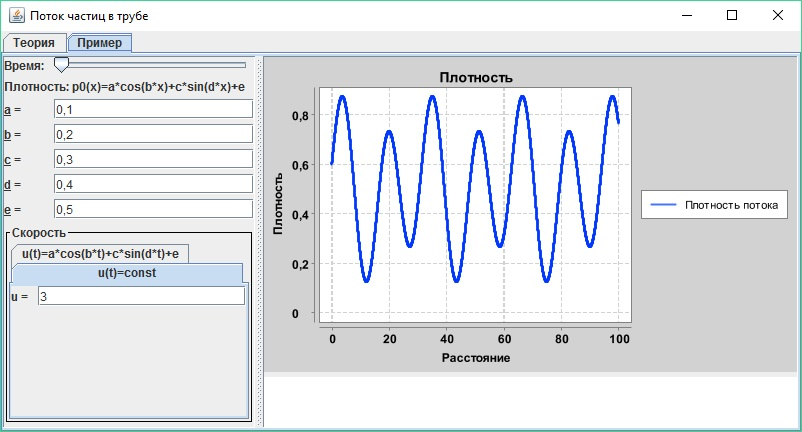
\includegraphics[width=0.7\linewidth]{images/tube_example}
			\caption{Интерактивная модель}
			\label{fig:tubeexample}
		\end{figure}
	

\chapter{Гидрологического барьера против загрязнения грунтовых вод}

	\section{Теоретическое введение}
		Снабжение крупных городов и промышленных центров доброкачественной водой для питья и водой для технических нужд давно стало острой техно-экологической проблемой. 
		Для ее решения помимо открытых и потому легко загрязняемых источников ( реки, озера, водохранилища) активно используются подземные воды влагосодержащих пластов. 
		Они менее подвержены антропогенным воздействиям, 	     однако и для них вопросы, связанные с зачастую неизбежным загрязнением, остаются актуальными. 
		Один из них – локализация вредных примесей, проникающих 	   в часть пласта с тем, чтобы вода в других частях оставалась чистой и пригодной для потребления.
		
		Эту цель можно достичь, используя часть грунтовых вод для создания на пути распространения загрязнений своебразного гидрологического барьера.
		
		Общая его схема показана  на рисунке \ref{fig:scheme}: между источником загрязнения (звездочки)        и водозаборными скважинами устанавливаются специальные скважины, накачивающие (достаточно чистую воду) воду в пласт и повышающие ее уровень ( барьер).
		\begin{figure}[th]
			\centering
			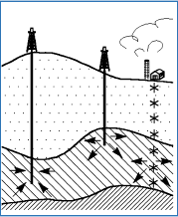
\includegraphics[width=0.4\linewidth]{images/scheme}
			\caption{Общая схема гидрологического барьера}
			\label{fig:scheme}
		\end{figure}
		
		Накачка создает принудительное движение грунтовых вод вправо и влево от барьера. Фильтрующая направо часть потока сносит назад текущую ей навстречу воду с примесями, препятствую дальнейшему продвижению загрязнений вдоль пласта.
		
		Математическая модель, реализующая эту схему, содержит уравнения фильтрации грунтовых вод 	 и уравнения распространения примесей, дополненные соответствующими входными данными (свойства грунта, воды и примесей).
		При относительно небольшом содержании примесей в воде они не оказывают на ее движение заметного влияния, и поэтому фильтрацию можно рассматривать отдельно  от динамики распространения загрязнений.
		
		При некоторых допущениях, главным из которых является предположение о достаточной протяженности пласта, движение воды описывается в рамках модели Буссинеска\cite{Samarskiy}:
		\begin{equation}
			\frac{\partial h}{\partial t}=k \frac{\partial}{\partial x}[(H(x,y)+h) \frac{\partial h}{\partial x}]+k\frac{\partial}{\partial y}[(H(x,y)+h)  \frac{\partial h}{\partial y}]
		\end{equation} 
		\begin{equation}
			k=\frac{\mu \rho g}{m},
		\end{equation} 
		
		где $ H $- функция поверхности пласта, $ h $-свободная поверхность воды.
		
		В этом случае все характеристики процесса – 		это функции переменных $ x $,$ y $,$ t $.
		
		Модель распространения примесей получается 	   (как и уравнение Буссинеска) из закона сохранения (баланса) массы примеси в элементе грунта. 
		Она представляет собой обычное уравнение неразрывности и в простейшем виде имеет вид:
		
		\begin{equation}
			\frac{\partial }{\partial t}[C(H+h)]+\frac{\partial}{\partial x}[C(H-h)u]+\frac{\partial}{\partial y}[C(H+h)\nu]=Q(x,y,t),
		\end{equation}
		
		где $ С(x,y,t) $ – искомая концентрация примесей, $ Q(x,y,t) $ – известная интенсивность источников загрязнений.
		
		Это уравнение можно также трактовать как двумерное уравнения переноса концентрации $ С $. Данное уравнение может быть записано в другой форме:
		
		\begin{equation}
			\frac{\partial }{\partial t}[C(H+h)]-\nu\frac{\partial}{\partial x}[C(H+h)\frac{\partial h}{\partial x}]-\nu\frac{\partial}{\partial y}[[C(H+h)\frac{\partial h}{\partial y}]=Q(x,y,t),
		\end{equation}
		
		так как по закону Дарси:
		
		\begin{equation}
			u=-v\frac{\partial h}{\partial x}, v=-\nu\frac{\partial h}{\partial y}, \nu=\mu\rho g.
		\end{equation}
	\section{Реализация}
	
		Реализация производилась на языке Java, версия 1.8. В программе присутствует секция с общей информацией о модели \ref{fig:barriertheory} и секция с интерактивным примером \ref{fig:barrierexample}, в которой дано графическое представление модели, а при изменении параметров появляются обучающие подсказки. Исходный код модели доступен на \href{https://github.com/goto1134/mathmodels}{GitHub}.
		
		\begin{figure}[th]
			\centering
			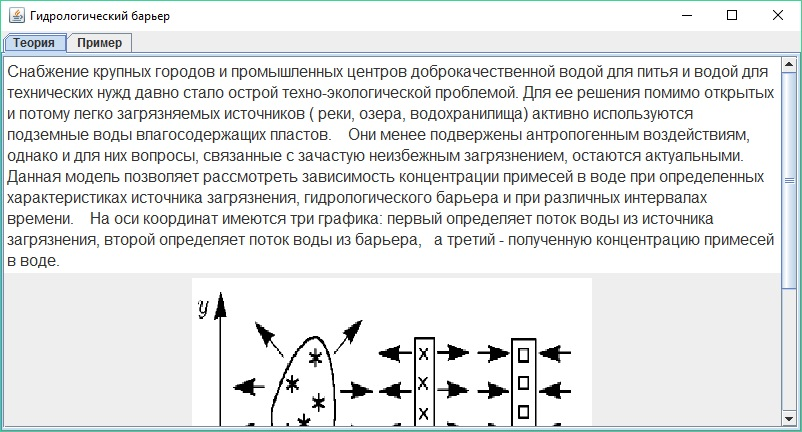
\includegraphics[width=0.7\linewidth]{images/barrier_theory}
			\caption{Общая информация о модели}
			\label{fig:barriertheory}
		\end{figure}
		\begin{figure}[th]
			\centering
			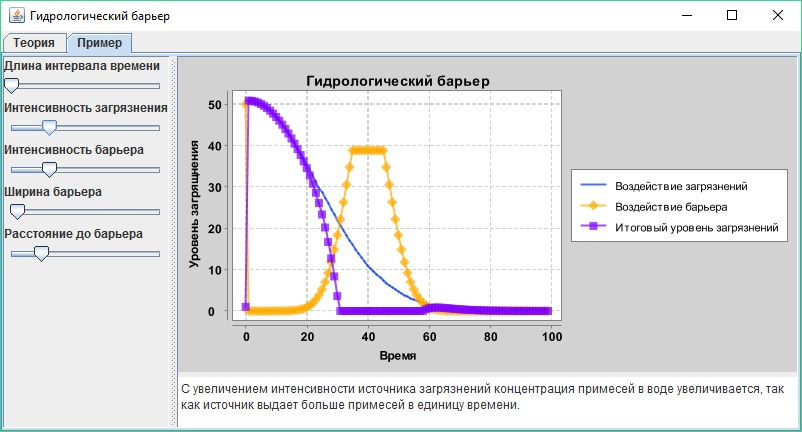
\includegraphics[width=0.7\linewidth]{images/barrier_example}
			\caption{Интерактивная модель}
			\label{fig:barrierexample}
		\end{figure}
		